\documentclass[11pt]{article}

\usepackage[a4paper,margin=0.85in]{geometry}
\usepackage{graphicx}
\usepackage{booktabs}
\usepackage{array}
\usepackage{longtable}
\usepackage{hyperref}
\usepackage{xcolor}
\usepackage{float}
\usepackage{enumitem}
\usepackage{caption}
\usepackage{subcaption}
\usepackage{microtype}

\hypersetup{
    colorlinks=true,
    linkcolor=blue!55!black,
    urlcolor=blue!55!black,
    citecolor=blue!55!black
}

\setlist[itemize]{topsep=3pt,itemsep=2pt,leftmargin=1.2em}
\setlist[enumerate]{topsep=3pt,itemsep=2pt,leftmargin=1.4em}
\renewcommand{\arraystretch}{1.15}

\title{\textbf{YouTube Speech Dataset Pipeline Report}\\
\large Source Curation, Clip Extraction, Quality Measurement, Transcript Repair, and Emotion Tagging}
\author{Sarvam Assignment Pipeline}
\date{June 2026}

\begin{document}
\maketitle

\begin{abstract}
This report documents a pipeline built to convert curated YouTube speech videos into reviewable Indian English and Hindi/code-mixed TTS training clips. The final run produced 188 matched before/after clip pairs totaling 61.11 minutes: 81 English clips and 107 Hindi clips. The strongest measured outcome was not acoustic denoising; it was dataset standardization and auditability. Final clips were aligned with raw source spans, converted to 24 kHz, loudness-normalized close to the -23 LUFS target, paired with transcripts, assigned traceable heuristic emotion/style tags, and exported with manual-review sheets and quality plots.

The main lesson from the iterations is that a pipeline can appear successful while still producing misleading metadata. The first dataset had source-quality issues. The second run exposed API quota/rate failures that silently collapsed semantic annotations to neutral/conversational. I fixed this by adding failure-aware metadata, transcript repair, stronger before/after metrics, and auditable emotion-tag repair with confidence and evidence fields.
\end{abstract}

\section{What I Built}

I built an end-to-end dataset preparation pipeline for extracting clean, single-speaker TTS clips from YouTube videos. The pipeline is designed around traceability: each final clip keeps pointers to the raw YouTube audio span, processed segment, transcript, source metadata, quality metrics, and review flags.

\subsection{Final Output}

\begin{table}[H]
\centering
\caption{Final dataset summary}
\begin{tabular}{lr}
\toprule
\textbf{Item} & \textbf{Value} \\
\midrule
Final clips & 188 \\
Matched raw before-clips & 188 \\
Total duration & 61.11 min \\
English clips & 81 \\
Hindi/code-mixed clips & 107 \\
Final sample rate & 24 kHz \\
Transcript coverage & 188 / 188 \\
Emotion/style status & Heuristic v2 with confidence/evidence \\
\bottomrule
\end{tabular}
\end{table}

\noindent The primary artifacts are:
\begin{itemize}
    \item \href{run:../data/metadata/10_final.jsonl}{\texttt{data/metadata/10\_final.jsonl}}: final clip metadata.
    \item \href{run:../analysis/before_after_manual_review.csv}{\texttt{analysis/before\_after\_manual\_review.csv}}: manual review sheet for raw/final clip pairs.
    \item \href{run:../analysis/before_after_metrics/before_after_report.md}{\texttt{analysis/before\_after\_metrics/before\_after\_report.md}}: audio before/after metrics.
    \item \href{run:../analysis/before_after_metrics/transcript_report.md}{\texttt{analysis/before\_after\_metrics/transcript\_report.md}}: transcript coverage and preservation metrics.
    \item \href{run:../analysis/emotion_tag_repair/emotion_tag_repair_report.md}{\texttt{analysis/emotion\_tag\_repair/emotion\_tag\_repair\_report.md}}: emotion tag repair report.
    \item \href{run:../packaged_artifacts/sarvam_code_methods_results_no_audio.zip}{\texttt{packaged\_artifacts/sarvam\_code\_methods\_results\_no\_audio.zip}}: code, methods, plots, and results without audio files.
\end{itemize}

\section{How the Pipeline Works}

\subsection{Pipeline Stages}

The pipeline is organized as a sequence of scripts under \href{run:../pipeline}{\texttt{pipeline/}}:

\begin{enumerate}
    \item \textbf{Source curation}: validates YouTube source metadata, expected language, speaker dominance, pre-listen quality, and prohibited source types.
    \item \textbf{Download}: downloads YouTube audio and converts it to 16 kHz mono WAV. A \texttt{pytubefix} fallback was added because \texttt{yt-dlp} was blocked on AWS for some videos.
    \item \textbf{Enhancement}: optionally runs enhancement. In this run, most sources were already clean and heavy enhancement was effectively not the measured win.
    \item \textbf{Diarization/transcription}: obtains diarized transcripts and word timestamps when API credits are available.
    \item \textbf{Macro extraction}: extracts speaker-homogeneous macro chunks from the diarized source.
    \item \textbf{VAD segmentation}: fragments macro chunks into 3--30 second clips and attaches approximate transcript spans.
    \item \textbf{DPBP boundary padding/trimming}: adjusts segment boundaries to reduce clipped starts/ends.
    \item \textbf{Speaker verification}: uses ECAPA similarity to retain clips consistent with the target speaker.
    \item \textbf{Quality filtering}: filters by duration, speaker verification, audio quality heuristics, language/script guardrails, clipping, and activity.
    \item \textbf{Emotion and text normalization}: assigns normalized transcript, emotion, and style. This stage was hardened after API failures.
    \item \textbf{Finalization}: exports final 24 kHz clips, matched raw before-clips, metadata, and review sheets.
\end{enumerate}

\subsection{Design Principle}

The most important design choice was to preserve provenance. A final clip is not just a WAV file; it carries:
\begin{itemize}
    \item source URL and source title,
    \item raw audio path,
    \item exact source start/end timestamps,
    \item processed segment path,
    \item final clip path,
    \item transcript fields,
    \item audio quality metrics,
    \item speaker verification score,
    \item emotion/style tag status,
    \item manual-review flags.
\end{itemize}

This made it possible to compare before and after clips, diagnose failures, and produce review-ready artifacts rather than only a folder of audio.

\section{Iterations and Improvements}

\subsection{Iteration 1: Initial Dataset}

The first iteration produced clips, but manual and automated inspection showed that the dataset was not acceptable. It contained language mismatches, read/voiceover-like speech, and clips that looked clean by basic script but were not ideal for expressive TTS training. The archived audit is documented in \href{run:../archive_one/iteration_1_audit_and_pipeline_hardening.md}{\texttt{archive\_one/iteration\_1\_audit\_and\_pipeline\_hardening.md}}.

\begin{table}[H]
\centering
\caption{Iteration 1 observations}
\begin{tabular}{p{0.31\linewidth}p{0.56\linewidth}}
\toprule
\textbf{Problem} & \textbf{Decision} \\
\midrule
Some Hindi clips had mostly English/Latin text & Add language/script guardrails and manual review flags. \\
Several clips sounded read, scripted, or voiceover-like & Add stricter source selection guardrails and source-type exclusions. \\
Raw vs processed trace was weak & Export matched raw spans for before/after review. \\
Quality decisions were hard to audit & Add CSV audits and rejection logs. \\
\bottomrule
\end{tabular}
\end{table}

\subsection{Iteration 2: Better Sources and Full Pipeline Run}

For the second iteration, I used a stronger curated source list with Indian English and Hindi/code-mixed speech. The pipeline produced 188 final clips and 188 matched raw before-clips. However, the run exposed a production issue: the Sarvam API hit quota/rate failures during semantic annotation. Previously, this failure could silently turn into valid-looking \texttt{neutral}/\texttt{conversational} labels.

\subsection{Pipeline Hardening}

The pipeline was improved in four main ways:
\begin{enumerate}
    \item \textbf{Source quality guardrails}: stronger source validation before downloading.
    \item \textbf{Before/after traceability}: each final clip now has a matched raw segment.
    \item \textbf{Failure-aware semantic metadata}: API failures are now explicit; they do not masquerade as valid labels.
    \item \textbf{Repair and measurement tools}: added transcript repair, audio metrics, ASR similarity measurement, and emotion tag repair.
\end{enumerate}

\section{Quality Metrics and Observations}

\subsection{Audio Before/After Metrics}

The before/after measurement showed a clear result: the pipeline standardized audio, but did not prove denoising or enhancement improvement.

\begin{table}[H]
\centering
\caption{Selected audio before/after metrics}
\begin{tabular}{lrrr}
\toprule
\textbf{Metric} & \textbf{Before/raw} & \textbf{After/final} & \textbf{Delta} \\
\midrule
Proxy SNR (dB) & 39.45 & 39.20 & -0.25 \\
Clipping (\%) & 0.0000 & 0.0000 & 0.0000 \\
Integrated loudness (LUFS) & -20.84 & -23.33 & -2.49 \\
LUFS target error vs -23 & +2.16 & -0.33 & improved \\
Peak dBFS & -3.34 & -5.56 & safer \\
Active speech ratio & 0.618 & 0.613 & -0.004 \\
Duration mismatch (sec) & -- & 0.0000 & exact \\
Acoustic similarity proxy & -- & 0.9912 & high preservation \\
\bottomrule
\end{tabular}
\end{table}

\begin{table}[H]
\centering
\caption{Quality gate summary}
\begin{tabular}{lr}
\toprule
\textbf{Gate} & \textbf{Result} \\
\midrule
SNR improved by more than 0.5 dB & 4.3\% \\
SNR unchanged within +/-0.5 dB & 71.8\% \\
SNR worsened by more than 0.5 dB & 23.9\% \\
Raw LUFS within 2 dB of -23 & 36.2\% \\
Final LUFS within 2 dB of -23 & 96.8\% \\
Duration delta under 50 ms & 100.0\% \\
Acoustic similarity at least 0.98 & 81.9\% \\
Final clips with zero clipping & 100.0\% \\
\bottomrule
\end{tabular}
\end{table}

\begin{figure}[H]
    \centering
    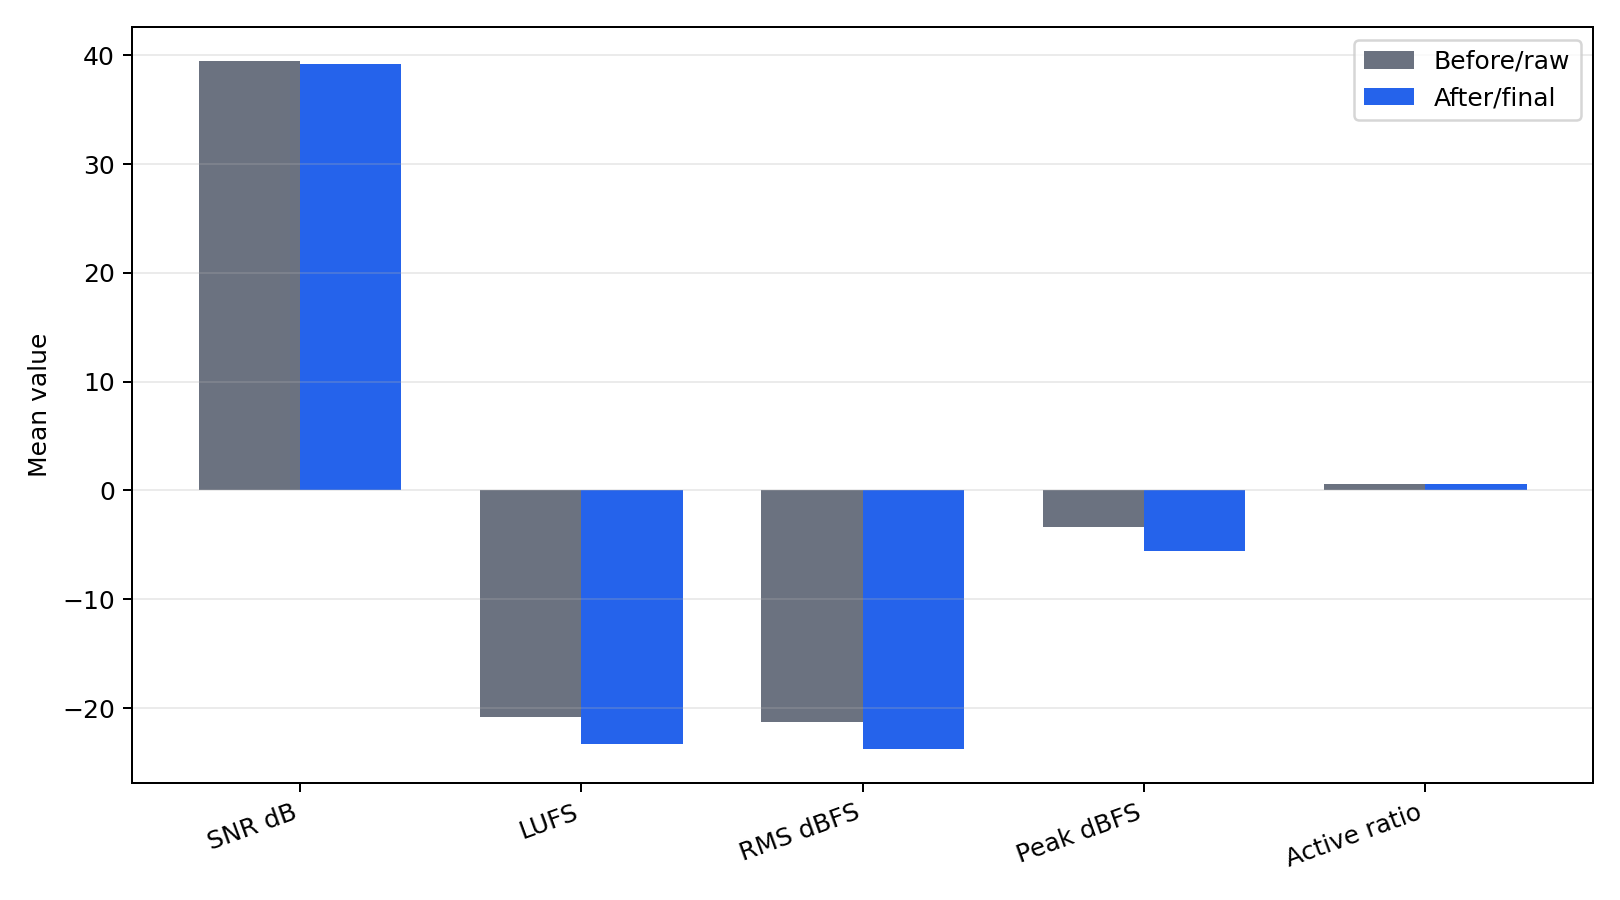
\includegraphics[width=0.88\linewidth]{quality_means_before_after.png}
    \caption{Mean audio metrics before and after finalization. The strongest effect is loudness/format standardization, not denoising.}
\end{figure}

\begin{figure}[H]
    \centering
    \begin{subfigure}{0.48\linewidth}
        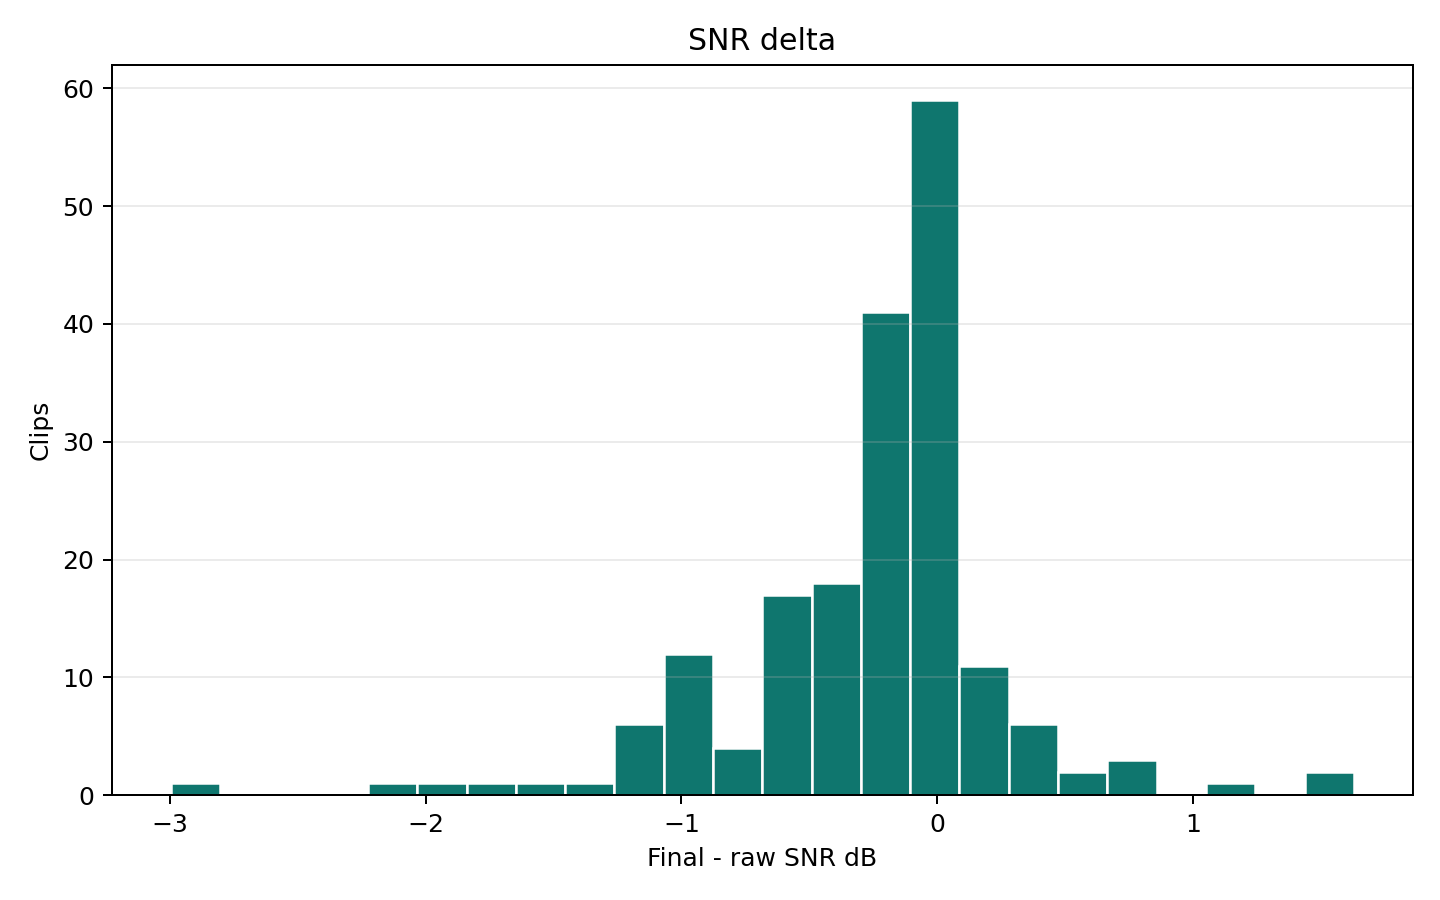
\includegraphics[width=\linewidth]{snr_delta_hist.png}
        \caption{SNR delta}
    \end{subfigure}
    \hfill
    \begin{subfigure}{0.48\linewidth}
        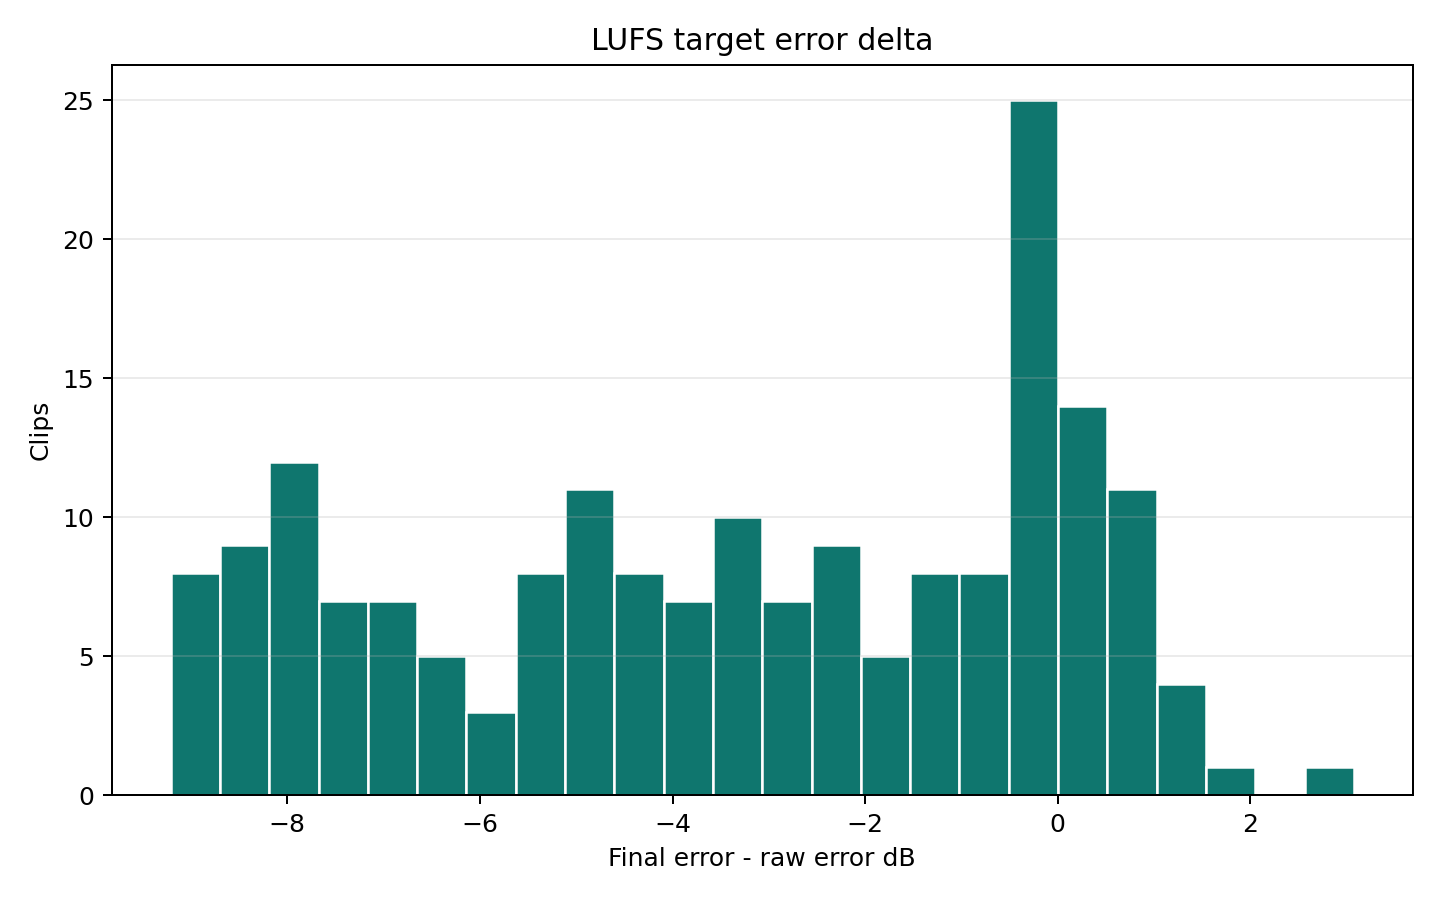
\includegraphics[width=\linewidth]{lufs_target_error_delta_hist.png}
        \caption{LUFS target error delta}
    \end{subfigure}
    \caption{SNR did not materially improve, while loudness moved closer to the target.}
\end{figure}

\begin{figure}[H]
    \centering
    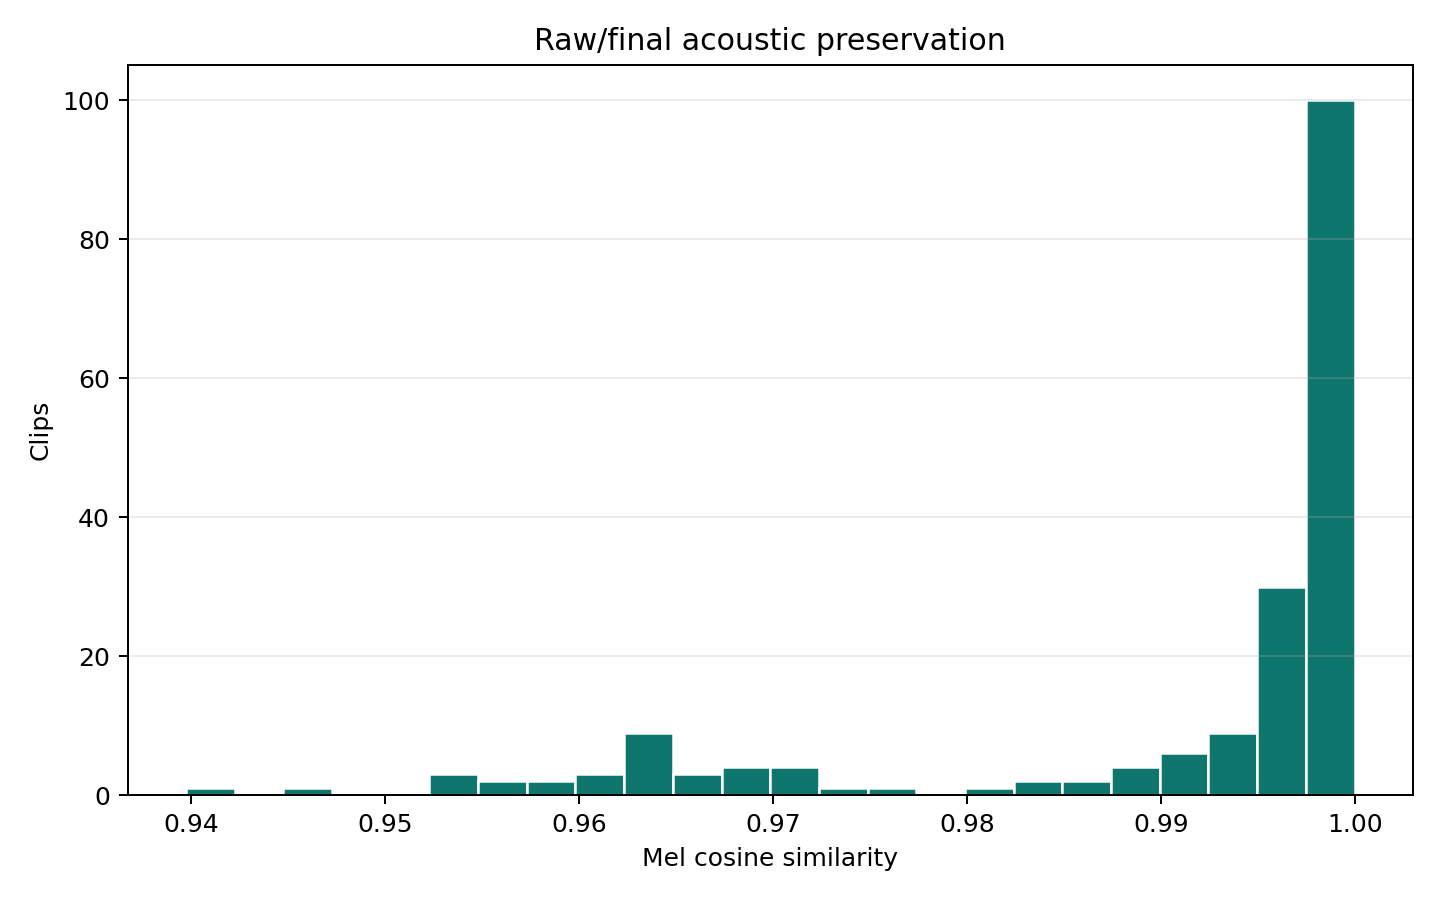
\includegraphics[width=0.78\linewidth]{acoustic_similarity_hist.png}
    \caption{Raw/final acoustic preservation. The high similarity confirms that finalization preserved the original spoken content.}
\end{figure}

\subsection{Interpretation}

The current evidence does \emph{not} support claiming that enhancement improved acoustic quality. The proxy SNR moved by -0.25 dB on average. This suggests that either the source audio was already clean enough that enhancement was unnecessary, or the enhancement stage did not materially alter the signal. The correct claim is narrower and more defensible:

\begin{quote}
The pipeline standardized clips for TTS dataset use: it created aligned raw/final pairs, converted final audio to 24 kHz, normalized loudness close to -23 LUFS, preserved duration alignment, avoided clipping, and retained high acoustic similarity.
\end{quote}

\section{Transcript Repair and Validation}

After the API failure, 110 clips were missing usable normalized transcripts. I repaired transcript coverage with local faster-whisper ASR and then measured raw-vs-final ASR similarity on the AWS GPU using faster-whisper \texttt{base}.

\begin{table}[H]
\centering
\caption{Transcript coverage}
\begin{tabular}{lr}
\toprule
\textbf{Item} & \textbf{Value} \\
\midrule
Final clips & 188 \\
Normalized transcripts present & 188 \\
Approx transcripts present & 188 \\
Local ASR-filled transcripts & 110 \\
Original pipeline transcripts & 78 \\
\bottomrule
\end{tabular}
\end{table}

\begin{table}[H]
\centering
\caption{Raw/final ASR preservation}
\begin{tabular}{lrrrr}
\toprule
\textbf{Split} & \textbf{Clips} & \textbf{Median char sim.} & \textbf{Median word F1} & \textbf{Word F1 < 0.90} \\
\midrule
All & 188 & 0.981 & 0.966 & 58 \\
English & 81 & 1.000 & 1.000 & 2 \\
Hindi/code-mixed & 107 & 0.900 & 0.884 & 56 \\
\bottomrule
\end{tabular}
\end{table}

\begin{figure}[H]
    \centering
    \begin{subfigure}{0.48\linewidth}
        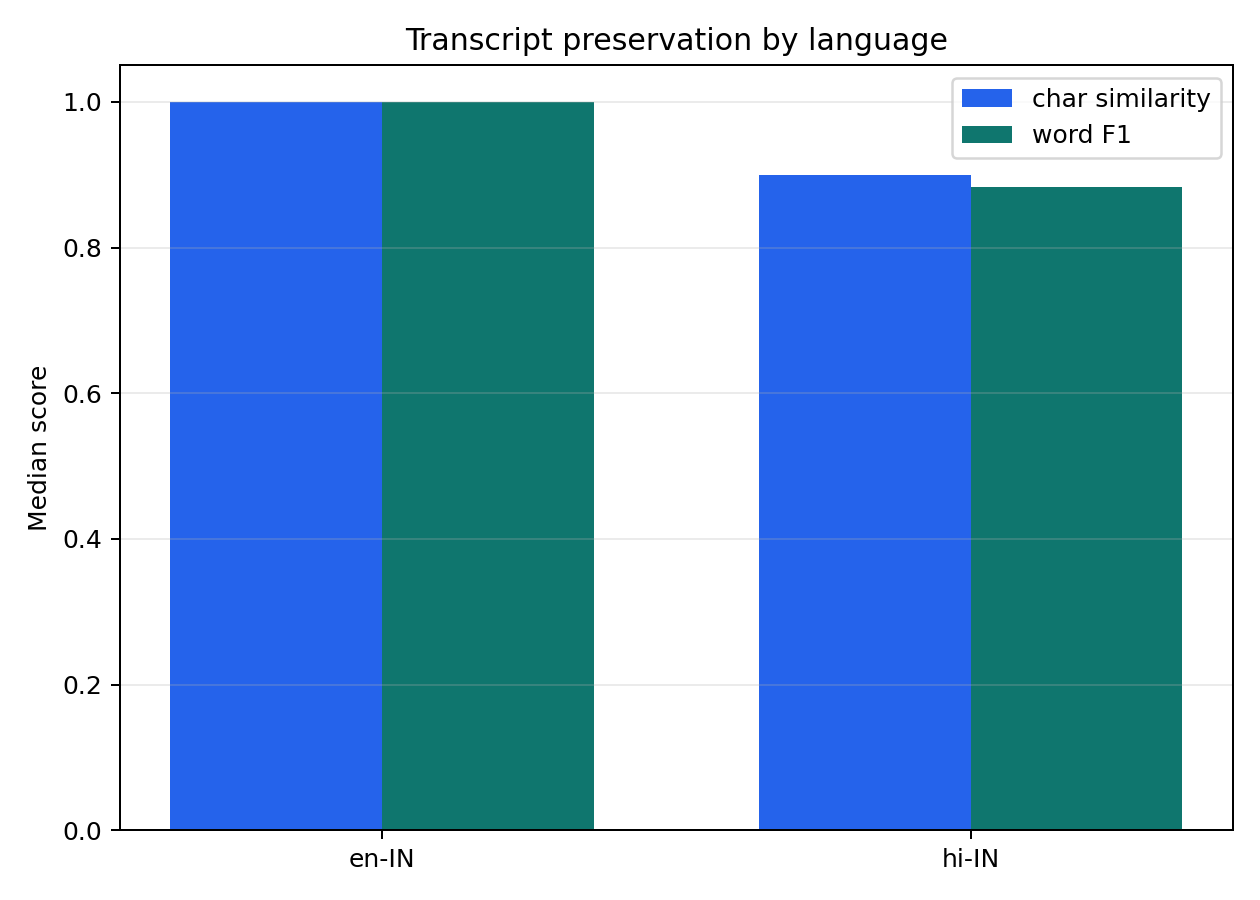
\includegraphics[width=\linewidth]{asr_similarity_by_language.png}
        \caption{Median similarity by language}
    \end{subfigure}
    \hfill
    \begin{subfigure}{0.48\linewidth}
        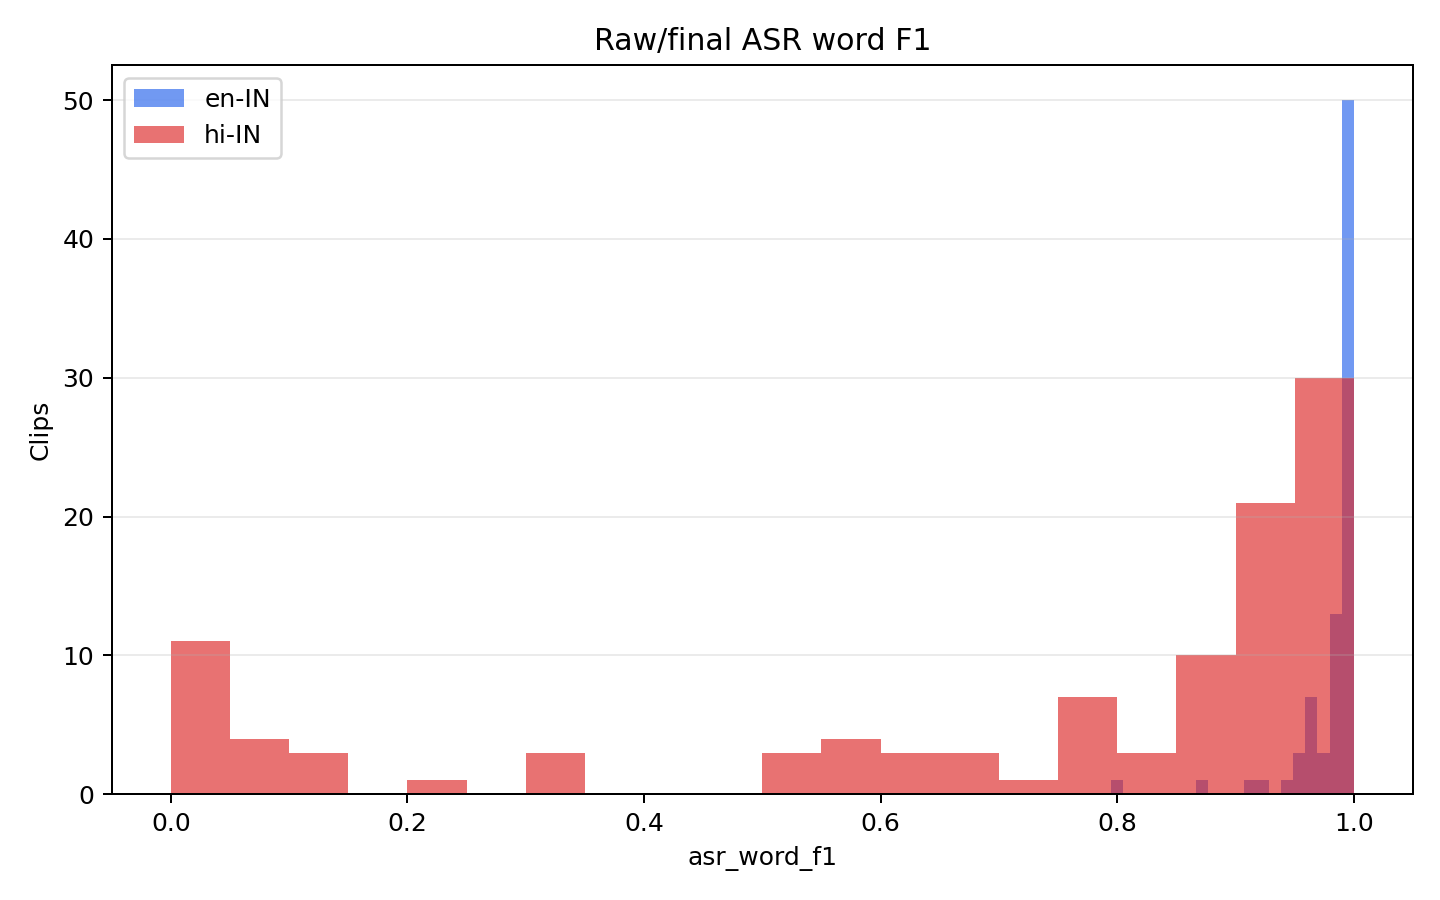
\includegraphics[width=\linewidth]{asr_word_f1_hist_by_language.png}
        \caption{ASR word F1 distribution}
    \end{subfigure}
    \caption{English ASR preservation is strong. Hindi/code-mixed ASR similarity is noisier and should be used as a manual-review priority signal.}
\end{figure}

\subsection{Transcript Decision}

The English preservation results are strong. The Hindi/code-mixed results are more complicated: many low-scoring rows show script instability in ASR output rather than obvious audio corruption. For this reason, I did not use the ASR similarity score as a hard rejection metric for Hindi. Instead, low-similarity rows are written to \href{run:../analysis/before_after_metrics/low_asr_similarity_review.csv}{\texttt{low\_asr\_similarity\_review.csv}} for manual review.

\section{Emotion and Style Tag Repair}

The original semantic stage failed because API quota/rate failures led to default-looking emotion/style fields. The first repair used source-level hints, but that was too coarse because it assigned many clips the same emotion from the whole video. The final repair, v2, retagged each clip using:

\begin{itemize}
    \item transcript keyword evidence,
    \item curated source emotion and register hints,
    \item clip-level speech rate,
    \item activity and loudness features,
    \item confidence and score margin thresholds.
\end{itemize}

These are still heuristic labels, not human labels and not trained emotion-model predictions. The repair is useful because it is auditable: each row includes \texttt{emotion\_confidence}, \texttt{emotion\_score\_margin}, \texttt{emotion\_evidence}, and \texttt{emotion\_review\_required}.

\begin{table}[H]
\centering
\caption{Emotion repair v2 summary}
\begin{tabular}{lr}
\toprule
\textbf{Item} & \textbf{Value} \\
\midrule
Clips retagged & 188 \\
Rows changed from previous heuristic & 57 \\
Manual review required & 68 \\
Mean confidence & 0.448 \\
\bottomrule
\end{tabular}
\end{table}

\begin{table}[H]
\centering
\caption{Final emotion and style distribution}
\begin{tabular}{lrlr}
\toprule
\textbf{Emotion} & \textbf{Clips} & \textbf{Style} & \textbf{Clips} \\
\midrule
Formal & 73 & Authoritative & 70 \\
Concerned & 48 & Conversational & 46 \\
Neutral & 46 & Formal & 39 \\
Sarcastic & 11 & Expressive & 33 \\
Excited & 10 & & \\
\bottomrule
\end{tabular}
\end{table}

\begin{figure}[H]
    \centering
    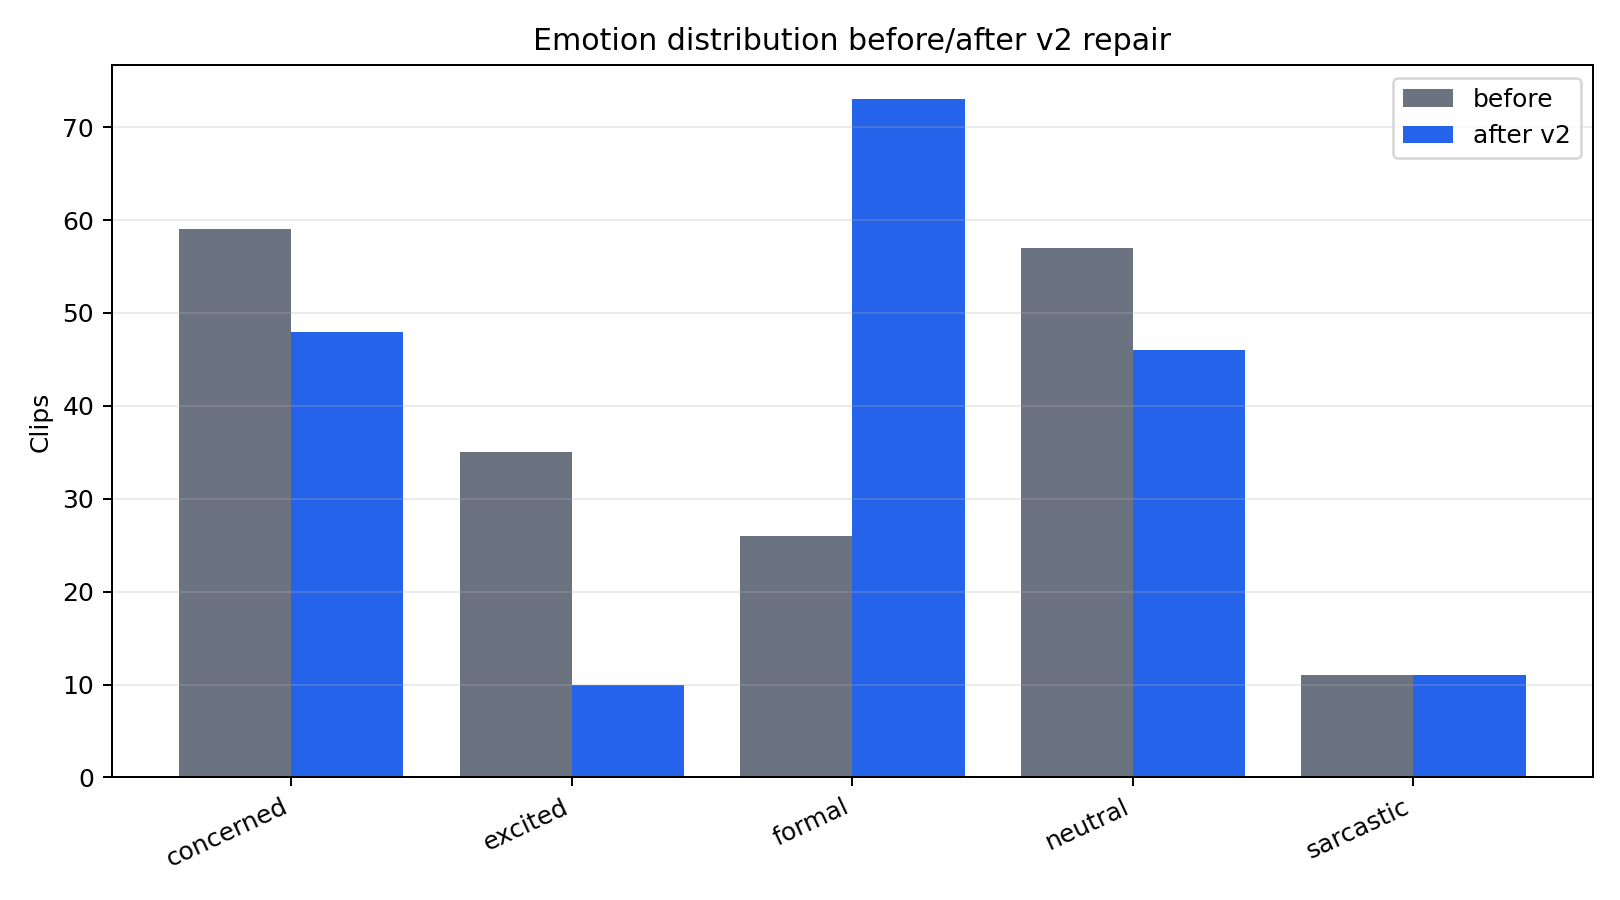
\includegraphics[width=0.86\linewidth]{emotion_distribution_before_after_v2.png}
    \caption{Emotion distribution before and after v2 repair. The repair reduced broad source-level over-assignment and moved lecture-like clips toward formal/authoritative labels.}
\end{figure}

\section{What Worked}

\begin{itemize}
    \item \textbf{Source curation improved the dataset}: the second source set produced a more useful pool of clips than the first iteration.
    \item \textbf{Traceability worked}: raw/final pairs made before/after measurement and manual review possible.
    \item \textbf{Speaker verification was effective as a major filter}: the rejection log was dominated by speaker similarity rejections, showing that speaker consistency mattered more than SNR in this run.
    \item \textbf{Finalization worked}: all final clips are 24 kHz, aligned with raw spans, zero-clipping, and close to the loudness target.
    \item \textbf{Transcript coverage was recovered}: final metadata now has transcripts for all 188 clips.
    \item \textbf{Failure-aware metadata improved reliability}: semantic failures are no longer hidden behind valid-looking labels.
\end{itemize}

\section{What Did Not Work}

\begin{itemize}
    \item \textbf{Enhancement did not measurably improve SNR}: the average proxy SNR delta was -0.25 dB, so I do not claim denoising improvement.
    \item \textbf{The SNR proxy is weak}: values around 39 dB are unusually high and should not be treated as perceptual quality or DNSMOS.
    \item \textbf{The semantic API stage was fragile}: API quota/rate failures caused missing transcripts and default semantic labels.
    \item \textbf{Hindi/code-mixed ASR similarity is noisy}: faster-whisper sometimes changes script/language between raw and final clips, so low ASR similarity needs manual review rather than automatic rejection.
    \item \textbf{Emotion tags are not ground-truth labels}: the final tags are auditable heuristics, not human annotations.
\end{itemize}

\section{Quality Decisions}

The main quality decisions I made were:

\begin{enumerate}
    \item \textbf{Do not overclaim enhancement}: report standardization and preservation, not denoising.
    \item \textbf{Keep low-confidence semantic rows}: instead of deleting them, expose review flags and confidence scores.
    \item \textbf{Use manual review where models are unreliable}: Hindi/code-mixed ASR and emotion tags need human verification.
    \item \textbf{Treat source choice as a first-class quality factor}: a clean pipeline cannot fully rescue poor sources.
    \item \textbf{Prefer traceability over black-box filtering}: every final clip can be traced back to its source span.
\end{enumerate}

\section{What I Would Improve With More Time}

\begin{itemize}
    \item Replace proxy SNR with stronger perceptual quality metrics such as DNSMOS, UTMOS, or a speech-aware SNR estimator.
    \item Add a human-labeled calibration set for emotion/style and report macro-F1 instead of relying on heuristics.
    \item Use a stronger Hindi/code-mixed ASR model or Sarvam ASR with sufficient credits to reduce transcript instability.
    \item Add automatic detection of read-aloud, dubbing, songs, and synthetic/robotic speech using classifiers rather than source text alone.
    \item Run A/B listening tests for a sample of raw vs final clips to validate whether loudness normalization improves usability.
    \item Add a small dashboard for manual review: play raw/final side by side, show transcript, emotion evidence, and one-click keep/reject labels.
    \item Improve the enhancement decision gate: only run Demucs/noise reduction when the source actually needs it, otherwise skip and mark the clip as already clean.
\end{itemize}

\section{Conclusion}

The final pipeline is useful because it produces a traceable, measurable, review-ready dataset rather than only extracted audio files. The strongest outcomes are clip extraction, speaker filtering, transcript recovery, loudness/format standardization, before/after measurement, and auditable semantic metadata.

The most important negative result is also valuable: the enhancement stage did not measurably improve audio quality in this run. That finding changed the interpretation of the pipeline from ``audio enhancement'' to ``dataset standardization and quality control.'' This is the kind of iteration that made the pipeline more honest and more production-ready.

\appendix
\section{Artifact Links}

\begin{itemize}
    \item Code and no-audio results archive: \href{run:../packaged_artifacts/sarvam_code_methods_results_no_audio.zip}{\texttt{packaged\_artifacts/sarvam\_code\_methods\_results\_no\_audio.zip}}
    \item Final metadata: \href{run:../data/metadata/10_final.jsonl}{\texttt{data/metadata/10\_final.jsonl}}
    \item Before/after metrics CSV: \href{run:../analysis/before_after_metrics/before_after_metrics.csv}{\texttt{analysis/before\_after\_metrics/before\_after\_metrics.csv}}
    \item Transcript similarity CSV: \href{run:../analysis/before_after_metrics/asr_text_similarity.csv}{\texttt{analysis/before\_after\_metrics/asr\_text\_similarity.csv}}
    \item Low transcript similarity review CSV: \href{run:../analysis/before_after_metrics/low_asr_similarity_review.csv}{\texttt{analysis/before\_after\_metrics/low\_asr\_similarity\_review.csv}}
    \item Emotion review CSV: \href{run:../analysis/emotion_tag_repair/emotion_manual_review_v2.csv}{\texttt{analysis/emotion\_tag\_repair/emotion\_manual\_review\_v2.csv}}
    \item Source list: \href{run:../sources/sources.jsonl}{\texttt{sources/sources.jsonl}}
    \item Iteration 1 audit: \href{run:../docs/iteration_1_audit_and_pipeline_hardening.md}{\texttt{docs/iteration\_1\_audit\_and\_pipeline\_hardening.md}}
\end{itemize}

\end{document}
